\documentclass{beamer}
\mode<presentation>
\usepackage{amsmath}
\usepackage{amssymb}
%\usepackage{advdate}
\usepackage{adjustbox}
\usepackage{subcaption}
\usepackage{enumitem}
\usepackage{multicol}
\usepackage{mathtools}
\usepackage{listings}
\usepackage{url}
\def\UrlBreaks{\do\/\do-}
\usetheme{Boadilla}
\usecolortheme{lily}
\setbeamertemplate{footline}
{
  \leavevmode%
  \hbox{%
  \begin{beamercolorbox}[wd=\paperwidth,ht=2.25ex,dp=1ex,right]{author in head/foot}%
    \insertframenumber{} / \inserttotalframenumber\hspace*{2ex} 
  \end{beamercolorbox}}%
  \vskip0pt%
}

\providecommand{\nCr}[2]{\,^{#1}C_{#2}} % nCr
\providecommand{\nPr}[2]{\,^{#1}P_{#2}} % nPr
\providecommand{\mbf}{\mathbf}
\providecommand{\pr}[1]{\ensuremath{\Pr\left(#1\right)}}
\providecommand{\qfunc}[1]{\ensuremath{Q\left(#1\right)}}
\providecommand{\sbrak}[1]{\ensuremath{{}\left[#1\right]}}
\providecommand{\lsbrak}[1]{\ensuremath{{}\left[#1\right.}}
\providecommand{\rsbrak}[1]{\ensuremath{{}\left.#1\right]}}
\providecommand{\brak}[1]{\ensuremath{\left(#1\right)}}
\providecommand{\lbrak}[1]{\ensuremath{\left(#1\right.}}
\providecommand{\rbrak}[1]{\ensuremath{\left.#1\right)}}
\providecommand{\cbrak}[1]{\ensuremath{\left\{#1\right\}}}
\providecommand{\lcbrak}[1]{\ensuremath{\left\{#1\right.}}
\providecommand{\rcbrak}[1]{\ensuremath{\left.#1\right\}}}
\theoremstyle{remark}
\newtheorem{rem}{Remark}
\newcommand{\sgn}{\mathop{\mathrm{sgn}}}
\providecommand{\abs}[1]{\left\vert#1\right\vert}
\providecommand{\res}[1]{\Res\displaylimits_{#1}} 
\providecommand{\norm}[1]{\lVert#1\rVert}
\providecommand{\mtx}[1]{\mathbf{#1}}
\providecommand{\mean}[1]{E\left[ #1 \right]}
\providecommand{\fourier}{\overset{\mathcal{F}}{ \rightleftharpoons}}
%\providecommand{\hilbert}{\overset{\mathcal{H}}{ \rightleftharpoons}}
\providecommand{\system}{\overset{\mathcal{H}}{ \longleftrightarrow}}
	%\newcommand{\solution}[2]{\textbf{Solution:}{#1}}
%\newcommand{\solution}{\noindent \textbf{Solution: }}
\providecommand{\dec}[2]{\ensuremath{\overset{#1}{\underset{#2}{\gtrless}}}}
\newcommand{\myvec}[1]{\ensuremath{\begin{pmatrix}#1\end{pmatrix}}}
\let\vec\mathbf

\lstset{
%language=C,
frame=single, 
breaklines=true,
columns=fullflexible
}

\numberwithin{equation}{section}

\lstset{
  language=Python,
  basicstyle=\ttfamily\small,
  keywordstyle=\color{blue},
  stringstyle=\color{orange},
  numbers=left,
  numberstyle=\tiny\color{gray},
  breaklines=true,
  showstringspaces=false
}

\title{Problem 1.9.12}
\author{ee25btech11023-Venkata Sai}

\date{\today} 
\begin{document}

\begin{frame}
\titlepage
\end{frame}

\section*{Outline}
\begin{frame}
\tableofcontents
\end{frame}
\section{Problem}
\begin{frame}
\frametitle{Problem Statement}
%
Find the length of the segment joining \textbf{A}$\brak{-6,7}$ and \textbf{B}$\brak{-1,-5}$. Also, find the
midpoint of AB. 
 \begin{table}[h!]    
  \centering
  

  \caption{Variables given}
  \label{tab 1.4.9.2}
\end{table}
\end{frame}

%\subsection{Literature}
\section{Solution}
\subsection{Formulas}
\setcounter{section}{1}
\begin{frame}
\frametitle{Formulas}
%\framesubtitle{Literature}
Formula:

The direction vector for the given two points $\vec{A}$ and $\vec{B}$ is given by $\vec{B}-\vec{A}$

Midpoint Formula:
\begin{align}
   \vec{P}=\frac{k(\vec{B})+(\vec{A})}{k+1}
\end{align}
Where: 

\centering{$k$ = 1 }

\begin{align}
\vec{A}=\myvec{-6\\7} \hspace{1cm} \vec{B}=\myvec{-1\\-5} 
\end{align}

\end{frame}
\subsection{Obtaining Length of the segment}
\begin{frame}
\frametitle{Obtaining Length of the segment}
    \begin{align}
\vec{B} - \vec{A} = \myvec{-1 - (-6) \\ -5 - 7} = \myvec{5 \\ -12}  
\end{align}
\begin{align}
d = \|\vec{B-A}\| = \sqrt{\brak{B-A}^\top \brak{B-A}} 
\end{align}
\begin{align}
\brak{\vec{B}-\vec{A}}^\top \brak{\vec{B}-\vec{A}}&=\myvec{5  \ -12}\myvec{5 \\ -12}\\
&=5\times5+-12\times-12 = 169\\
d &=\sqrt{169}=13
\end{align}
Hence, the length of the segment $\vec{AB}$ is 13 units.
\end{frame}
\subsection{Finding Midpoint}
\begin{frame}
\frametitle{Finding Midpoint}

\begin{align}
\vec{P}=\frac{\vec{B}+\vec{A}}{2}=\frac{\myvec{-6\\7}+\myvec{-1\\-5}}{2}&=\frac{\myvec{-7\\2}}{2}\\ &=\myvec{\frac{-7}{2}\\1}
\end{align}

Hence the coordinates of $\vec{P}$ are $\brak{\frac{-7}{2},1}$



\end{frame}

\subsection{Plot}
\begin{frame}[fragile]
\frametitle{Plot}

\begin{figure}[H]
   \centering
   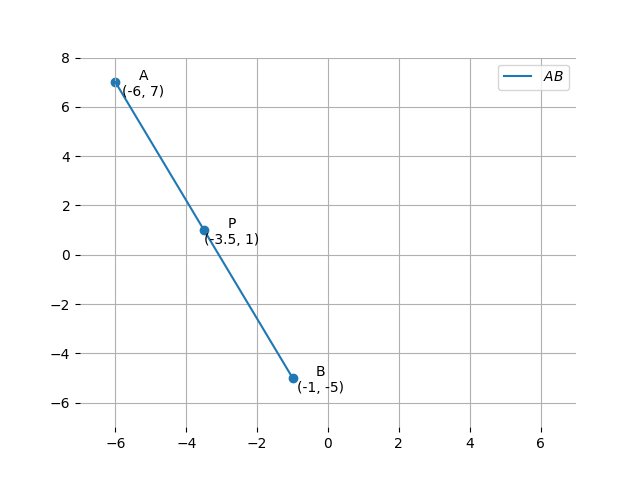
\includegraphics[width=0.8\columnwidth]{figs/fig1.png}
	\caption{}
   \label{stemplot}
\end{figure}
\end{frame}

\section{C Code}
\begin{frame}[fragile]
\frametitle{C Code for generating points on line}
\begin{lstlisting}[language=C]
#include <math.h>
#include <stdio.h>
#include <stdlib.h>
#include <string.h>
#include <unistd.h>
#include <sys/socket.h>
#include <netinet/in.h>

#include "libs/matfun.h"
#include "libs/geofun.h"

int main() {
    double **k, **M, **C;
     int x1 = -6, x2 = -1, y1 = 7, y2 = -5;

    // Create matrices
    M = createMat(2, 2);
    k = createMat(2, 1);
    C = createMat(2, 1);
 
    \end{lstlisting}
\end{frame}
\begin{frame}[fragile]
\frametitle{C Code for generating points on line}
\begin{lstlisting}[language=C]
  M[0][1] = x1;  
    M[1][1] = y1;  


    M[0][0] = x2;  
    M[1][0] = y2;  

 
    k[0][0] =1.0 / 2;  // weight for B (column 0)
    k[1][0] = 1.0 / 2;  // weight for A (column 1)

    // Matrix multiplication: C = M * k
    C = Matmul(M, k, 2, 2, 1);

    // Write result to file
    FILE *file = fopen("values.dat", "w");
    if (file == NULL) {
        printf("Error opening file!\n");
        return 1;
\end{lstlisting}
\end{frame}

\begin{frame}[fragile]
\frametitle{C Code for generating points on line}
\begin{lstlisting}[language=C]
     }
      fprintf(file, "x\ty\t of C\n");
    fprintf(file, "%.02lf\t%.02lf\n", C[0][0], C[1][0]);  // x and y of C

    fclose(file);
    printf("Results have been written to values.dat\n");

    // Free memory
    freeMat(M, 2);
    freeMat(k, 2);
    freeMat(C, 2);

    return 0;
}
\end{lstlisting}
\end{frame}

\section{Python Code}
\begin{frame}[fragile]
\frametitle{Python Code for Plotting}
\begin{lstlisting}[language=Python]
# Code by /sdcard/github/matgeo/codes/CoordGeoVV Sharma
# September 12, 2023
# Revised July 21, 2024
# Released under GNU GPL
# Section Formula

import sys
sys.path.insert(0, '/workspaces/urban-potato/matgeo/codes/CoordGeo/')  # path to my scripts
import numpy as np
import matplotlib.pyplot as plt
import matplotlib.image as mpimg
# Local imports
from line.funcs import *
from triangle.funcs import *
from conics.funcs import circ_gen

\end{lstlisting}
\end{frame}

\begin{frame}[fragile]
\frametitle{Python Code for Plotting}
\begin{lstlisting}[language=Python]
# Read data
data = np.loadtxt("values.dat", skiprows=1)

xc = data[0]  # Extract x-coordinate (e.g., -1)
yc = data[1]  # Extract y-coordinate (e.g., 4.5)

# Given points
A = np.array([-6, 7]).reshape(-1, 1)
B = np.array([-1, -5]).reshape(-1, 1)
P = np.array([xc, yc]).reshape(-1, 1)

# Generating line AB
x_AB = line_gen(A, B)

# Plotting
plt.plot(x_AB[0, :], x_AB[1, :], label='$AB$')

\end{lstlisting}
\end{frame}

\begin{frame}[fragile]
\frametitle{Python Code for Plotting}
\begin{lstlisting}[language=Python]
# Labeling the coordinates
tri_coords = np.block([[A, B, P]])
plt.scatter(tri_coords[0, :], tri_coords[1, :])

vert_labels = ['A', 'B', 'P']

# Helper function: format number with decimal only if needed
def fmt(val):
    return f"{val:.1f}" if abs(val - round(val)) > 1e-6 else f"{int(val)}"

for i, txt in enumerate(vert_labels):
    x = tri_coords[0, i].item()
    y = tri_coords[1, i].item()
    plt.annotate(f'{txt}\n({fmt(x)}, {fmt(y)})',
                 (x, y),
                 textcoords="offset points",
                 xytext=(20, -10),
                 ha='center')
\end{lstlisting}
\end{frame}

\begin{frame}[fragile]
\frametitle{Python Code for Plotting}
\begin{lstlisting}[language=Python]
ax = plt.gca()
ax.spines['left'].set_visible(False)
ax.spines['right'].set_visible(False)
ax.spines['top'].set_visible(False)
ax.spines['bottom'].set_visible(False)

plt.legend(loc='best')
plt.grid()

# Increase y-axis from -8 to 8 to show full range
plt.ylim(-7, 8)
plt.xlim(-7,7)

# Save and open
plt.show()
plt.savefig('../figs/fig1.png')
\end{lstlisting}
\end{frame}

\end{document}
